
% 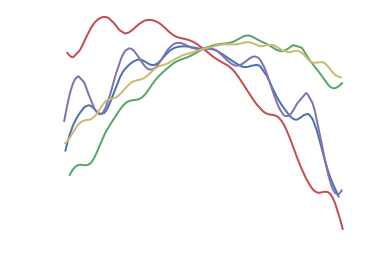
\includegraphics[width=.153\textwidth]{figs/gpSamples/main.png}
\begin{tikzpicture}


% level 1
\node (hyp) {\normalsize \color{blue} What is the probability of a trend, a recurring pattern {\bf and} noise in the data?};
\node[below = -0.2cm of hyp, text width =\textwidth,
align=center,font=\footnotesize] (hyp_form)
{$P\big((\LINK\lor\LINK\times\SEK)\;\land\;
(\PERK\lor\PERK\times\SEK\lor\PERK\times\LINK)$ 

$\; \land \; (\WNK\lor\LINK\times\WNK) \mid \xbf,\ybf, \thetabf \big) = 0.36$};

%level 2
\node[below =.5cm of hyp_form , xshift=-3.5cm] (trend) {\color{blue} Is there a trend?};
\node[below = -0.2cm of trend] (trend_form) {\scriptsize$P(\LINK\lor\LINK\times\SEK  \mid \xbf,\ybf, \thetabf ) = 0.65$};
\node[below = -0.2cm of trend_form] (trend_png) {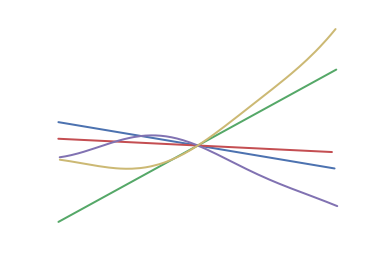
\includegraphics[width=.15\textwidth]{figs/gpSamples/trend.png}};

\node[below =.5cm of hyp_form, xshift=3.5cm] (noise) {\color{blue} Is there noise? };
\node[below = -0.2cm of noise] (noise_form) {\scriptsize$P(\WNK\lor\LINK\times\WNK  \mid \xbf,\ybf, \thetabf ) = 0.75$};
\node[below = -0.2cm of noise_form] (noise_png) {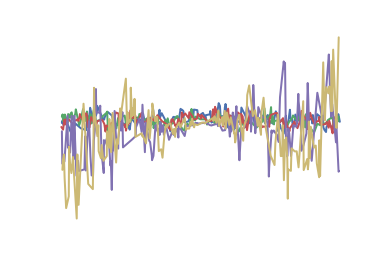
\includegraphics[width=.15\textwidth]{figs/gpSamples/noise.png}};

% level 3
\node[below =.5cm of trend_png , xshift=-2.6cm] (linear_trend) {\color{blue} A linear trend?};
\node[below = -0.2cm of linear_trend] (linear_trend_form) {\tiny$P(\LINK  \mid \xbf,\ybf, \thetabf ) = 0.63$};
\node[below = -0.2cm of linear_trend_form] (linear_trend_png) {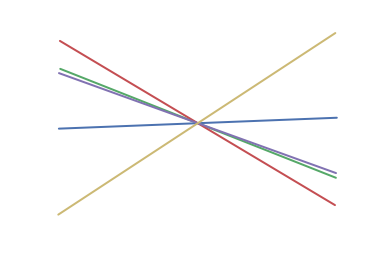
\includegraphics[width=.15\textwidth]{figs/gpSamples/lin.png}};

\node[below =.5cm of trend_png , xshift=1.2cm] (smooth_trend) {\color{blue} A smooth trend?};
\node[below = -0.2cm of smooth_trend] (smooth_trend_form) {\tiny$P(\LINK\times\SEK  \mid \xbf,\ybf, \thetabf ) = 0.02$};
\node[below = -0.2cm of smooth_trend_form] (smooth_trend_png) {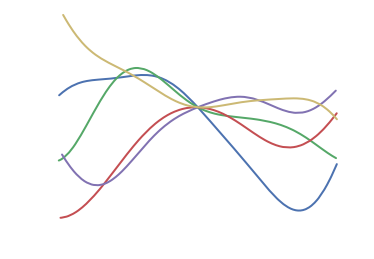
\includegraphics[width=.15\textwidth]{figs/gpSamples/selin.png}};

\node[below =.5cm of noise_png, xshift=-1.2cm] (het_noise) {\color{blue} Heteroskedastic noise? };
\node[below = -0.2cm of het_noise] (het_noise_form) {\tiny$P(\LINK\times\WNK  \mid \xbf,\ybf, \thetabf ) = 0$};
\node[below = -0.2cm of het_noise_form] (het_noise_png) {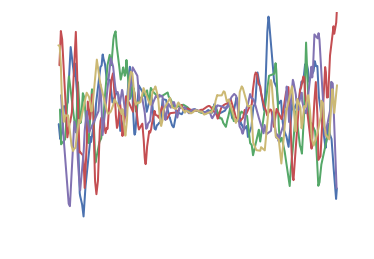
\includegraphics[width=.15\textwidth]{figs/gpSamples/linwn.png}};

\node[below =.5cm of noise_png, xshift=2.6cm] (white_noise) {\color{blue} White  noise? };
\node[below = -0.2cm of white_noise] (white_noise_form) {\tiny$P(\WNK  \mid \xbf,\ybf, \thetabf ) = 0.75$};
\node[below = -0.2cm of white_noise_form] (white_noise_png) {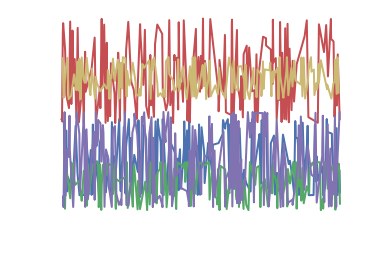
\includegraphics[width=.15\textwidth]{figs/gpSamples/wn.png}};

% level 4
\node[below =6.8cm of hyp_form] (recurring) {\color{blue} Is there repeating structure?};
\node[below = -0.2cm of recurring] (recurring_form) {\scriptsize$P(\PERK\lor\PERK\times\SEK\lor\PERK\times\LINK  \mid \xbf,\ybf, \thetabf ) = 0.73$};
\node[below = -0.2cm of recurring_form] (recurring_png) {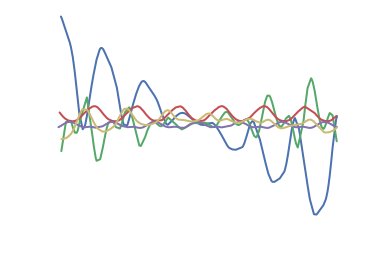
\includegraphics[width=.15\textwidth]{figs/gpSamples/recurring.png}};
%\draw[->,dashed] (barplot) -- (mcmc);

% level 5
\node[below =.5cm of recurring_png] (seper_form) {\scriptsize$P(\PERK\times\SEK
\mid \xbf,\ybf, \thetabf )=0.34\;\;\;\;\;\;$};
\node[below = -0.2cm of seper_form] (seper_png) {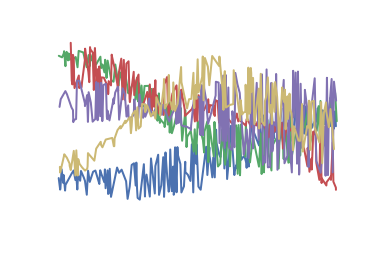
\includegraphics[width=.15\textwidth]{figs/gpSamples/seper.png}};

\node[below =.5cm of recurring_png, xshift=-4.7cm] (per_form) {\scriptsize$P(\PERK  \mid \xbf,\ybf, \thetabf )=0.32$};
\node[below = -0.2cm of per_form] (per_png) {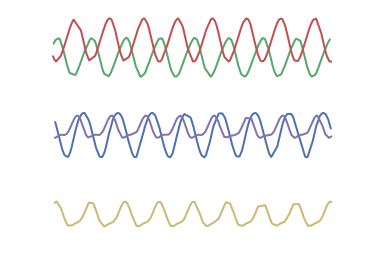
\includegraphics[width=.15\textwidth]{figs/gpSamples/per.png}};

\node[below =.5cm of recurring_png,xshift=4.7cm] (perlin_form)
{\scriptsize$P(\PERK\times\LINK  \mid \xbf,\ybf, \thetabf )=0.07$};
\node[below = -0.2cm of perlin_form] (seper_png) {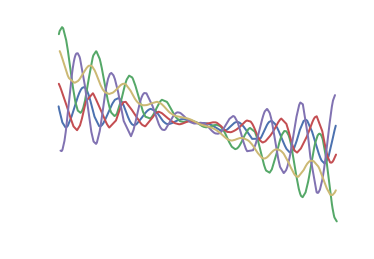
\includegraphics[width=.15\textwidth]{figs/gpSamples/perlin.png}};





\draw[->] (hyp_form) -- (trend);
\draw[->] (hyp_form) -- (noise);
\draw[->] (hyp_form) -- (recurring);


\draw[->] (noise_png) -- (het_noise);
\draw[->] (noise_png) -- (white_noise);

\draw[->] (trend_png) -- (linear_trend);
\draw[->] (trend_png) -- (smooth_trend);

\draw[->] (recurring_png) -- (per_form);
\draw[->] (recurring_png) -- (seper_form);
\draw[->] (recurring_png) -- (perlin_form);


\end{tikzpicture}



%  \multicolumn{3}{c}{\scriptsize$P(\PERK\lor\PERK\times\SEK\lor\PERK\times\LINK)$}
